\section{secret$\_$phase}
	此时的炸弹还没有拆完。根据前人的经验,这里还有一个隐藏关等着破解。
	
\subsection{find the secret phase}
	\begin{itemize}
	
	\item
	
	首先考虑如何进入隐藏关。由于每次拆弹成功都需要调用\textbf{phase$\_$defused}函数,想进入新的关卡,突破口肯定在这个函数。函数的代码如下:
	
	\lstinputlisting[language={[x86masm]Assembler}]{sources/phase_defused.asm}

	\item
		
	观察这个函数,发现这里调用了\textbf{secret$\_$phase}函数。
	
	\lstinputlisting[language={[x86masm]Assembler}]{sources/phase_defused_part_1.asm}
	
	这段语句是在第四关拆炸弹成功后执行,
	若要跳转到\textbf{secret$\_$phase}语句,需要以下两个条件:
	\begin{itemize}
		\item	由\textbf{cmp $\$0x2, \%eax$}看出,需要输入两个参数
		\item	这里调用了\textbf{strings$\_$not$\_$equal}函数,输入的第二个参数要与\textbf{0x8049dd2}中的值一样。
	\end{itemize}

	\item	
	于是调用gdb,查看\textbf{0x8049dd2}中的值:
	
	\begin{figure}[h]
		\centering
			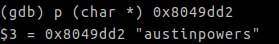
\includegraphics[scale=0.8]{images/phase_defused_part_2.png}
	\end{figure}	

	这样进入隐藏关的方法就很清楚了:在解锁第四关时输入\textbf{5 austinpowers},进入隐藏关。

	\end{itemize}
	
\subsection{solve the secret phase}
	\begin{itemize}
	
	\item
	
	隐藏关的代码如下:
	
	\lstinputlisting[language={[x86masm]Assembler}]{sources/secret_phase.asm}

	\item
	
	这里也调用了\textbf{strtol}函数,用处也相同:将输入的字符串转换为10进制整数。

	\lstinputlisting[language={[x86masm]Assembler}]{sources/secret_phase_part_1.asm}

	\item
		
	\lstinputlisting[language={[x86masm]Assembler}]{sources/secret_phase_part_2.asm}

	这里表示,我们输入的整数必须要不大于\textbf{0x3e9}。
	
		\lstinputlisting[language={[x86masm]Assembler}]{sources/secret_phase_part_3.asm}

	这一段表示,程序将存在\textbf{0x804c0c0}处的数据作为参数,传入\textbf{fun7}函数中。如果\textbf{fun7}的返回值不为7,炸弹爆炸。
	
	\item
	
	因此,我们的目标就是:找出使\textbf{fun7}的返回值为7的输入参数。

	\item
	
	\textbf{fun7}的代码如下:
	
	\lstinputlisting[language={[x86masm]Assembler}]{sources/fun_7.asm}

	这段代码的等价c语言表示如下:

	\lstinputlisting{sources/fun7.txt}
	
	
	
	这个可以理解为一个在一个二叉查找树中查找值的过程,从根开始,如果向右走,当前位就是1,向左走就是0。由于输出需要为7,因此需要向右走3次。

	\newpage

	\item
		
	首先通过gdb得出这一条路上的所有节点:

	\begin{figure}[h]
		\centering
			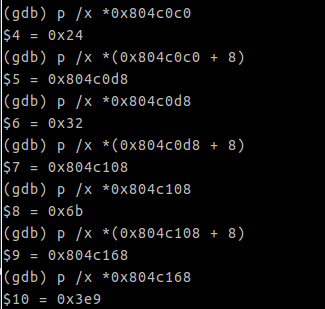
\includegraphics[scale=0.7]{images/secret_phase_part_4.png}
	\end{figure}	

	\item
			
	于是得出对应的二叉查找树:
	
	\begin{figure}[h]
		\centering
			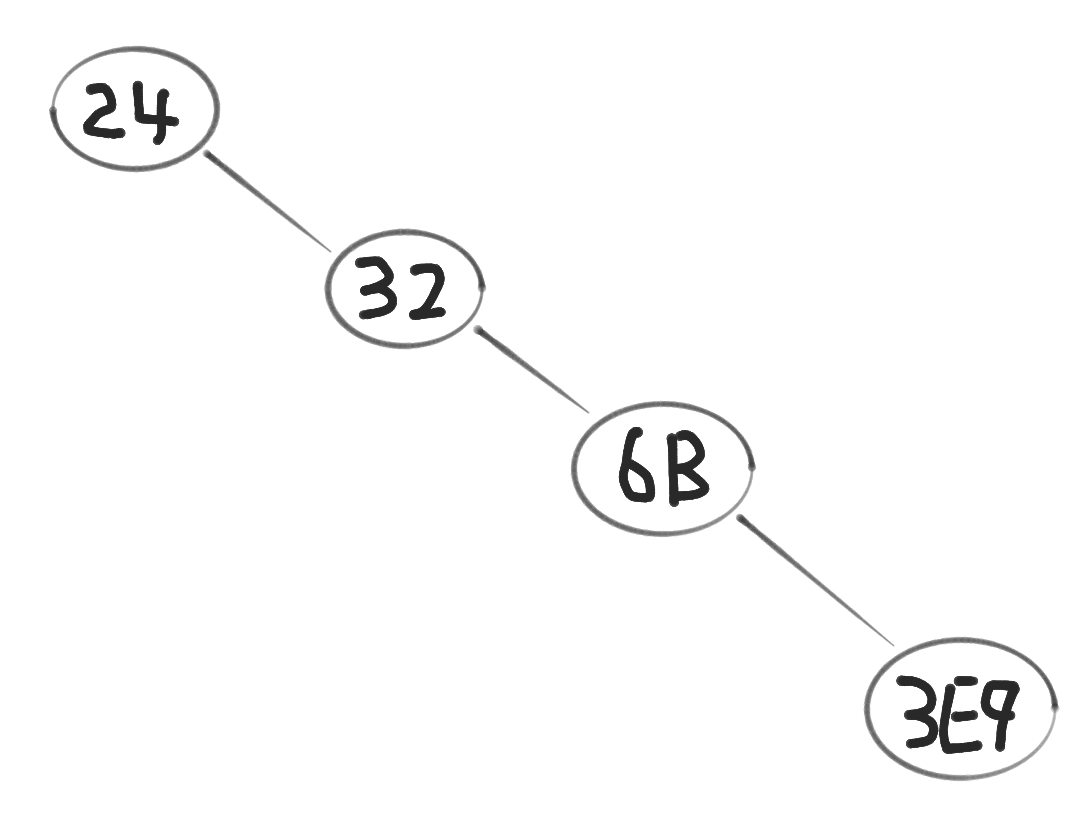
\includegraphics[scale=0.27]{images/secret_phase_part_5.png}
	\end{figure}	
	
	\item
	
	所以我们输入的值就是\textbf{0x3e9},转换为十进制就是1001。
	
	\end{itemize}		
	
	\newpage
	
	输入1001,问题解决。
	
	\begin{figure}[h]
		\centering
			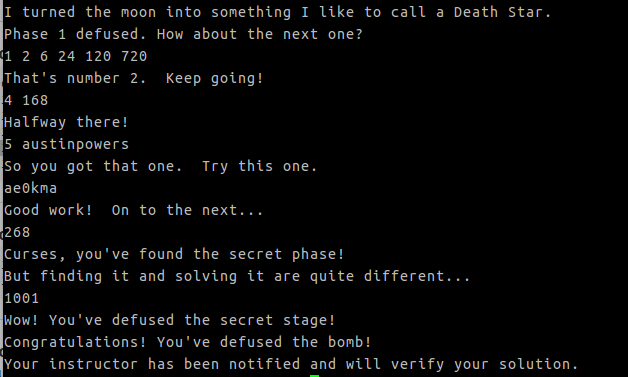
\includegraphics[scale=0.77]{images/secret_phase.success.png}
	\end{figure}	